
\documentclass[tikz,border=2mm]{standalone}
\usepackage[utf8]{inputenc}
\usepackage[T1]{fontenc}
\usepackage{amsmath}
\usepackage{amssymb}
\usetikzlibrary{arrows.meta,positioning,calc,shapes.geometric}
\usepackage{xcolor}

\definecolor{inkNavy}{HTML}{1B2733}
\definecolor{slate}{HTML}{3B4B5C}
\definecolor{paper}{HTML}{FBFAF7}
\definecolor{amber}{HTML}{C97A2B}
\definecolor{teal}{HTML}{2E7D74}
\definecolor{softred}{HTML}{A6402F}
\definecolor{lightgrey}{HTML}{E7E4DD}
\definecolor{midgrey}{HTML}{8B8A85}

\begin{document}
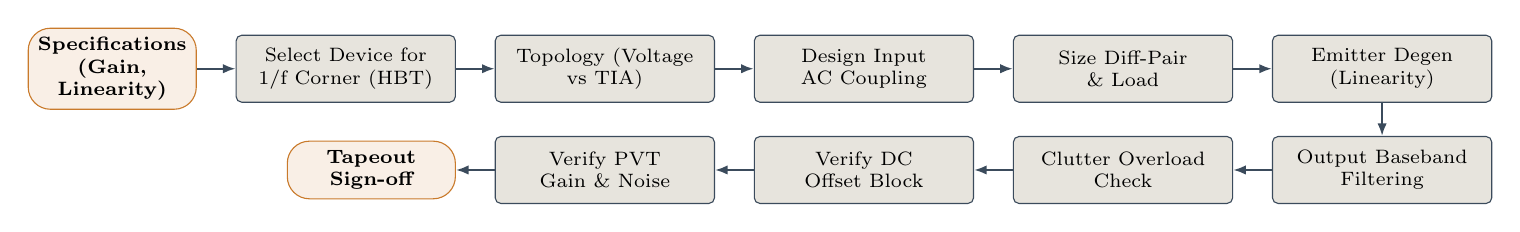
\begin{tikzpicture}[
  node distance=6pt and 14pt,
  box/.style={draw=slate, fill=lightgrey, rounded corners=2pt, text width=2.55cm, align=center, minimum height=0.85cm, font=\scriptsize},
  term/.style={draw=amber, fill=amber!12, rounded corners=8pt, text width=1.9cm, align=center, minimum height=0.7cm, font=\scriptsize\bfseries},
  arr/.style={-{Latex[length=1.6mm]}, slate, thick}
]
\node[term] (spec) {Specifications\\(Gain, Linearity)};
\node[box, right=of spec] (noise) {Select Device for\\1/f Corner (HBT)};
\node[box, right=of noise] (top) {Topology (Voltage\\vs TIA)};
\node[box, right=of top] (ac) {Design Input\\AC Coupling};
\node[box, right=of ac] (core) {Size Diff-Pair\\\& Load};
\node[box, right=of core] (degen) {Emitter Degen\\(Linearity)};

\node[box, below=12pt of degen] (filter) {Output Baseband\\Filtering};
\node[box, left=of filter] (clip) {Clutter Overload\\Check};
\node[box, left=of clip] (dc) {Verify DC\\Offset Block};
\node[box, left=of dc] (pvt) {Verify PVT\\Gain \& Noise};
\node[term, left=of pvt] (fin) {Tapeout\\Sign-off};

\draw[arr] (spec)--(noise); \draw[arr] (noise)--(top); \draw[arr] (top)--(ac);
\draw[arr] (ac)--(core); \draw[arr] (core)--(degen); \draw[arr] (degen)--(filter);
\draw[arr] (filter)--(clip); \draw[arr] (clip)--(dc); \draw[arr] (dc)--(pvt);
\draw[arr] (pvt)--(fin);
\end{tikzpicture}
\end{document}